\documentclass{assignment}
\usepackage{amsmath}
\usepackage{graphicx}
\usepackage{paracol}
\begin{document}
\title{Assignment 1}
\author{NYALAPOGULA MANASWINI(CS20btech11035)}
\maketitle
\begin{paracol}{2}
\switchcolumn[0]
\begin{Large}
QUESTION 3.3:\\
Suppose X has a binomial\\
 distribution . Show that X = 3 is the most likely outcome.(Hint : P(X = 3) is the maximum among all P($x_i$), ($x_i$= 0,1,2,3,4,5,6).\\Assume p=0.5\\ 
 \\
SOLUTION:\\
Let X be a binomial random \\variable which has probability p=0.5\\
Given number of times event(X) is\\
 performed(n)=6\\
Given probability of event(p)=0.5\\
Therefore probability that event(X)\\ does not occur is
(1-p)=1-0.5=0.5\\
We know that binomial probability\\
\begin{equation}
P(X=k)= \binom{n}{k}p^k({1-p})^{n-k}  \label{1} 
\end{equation}
For P(X=k) to be most likely\\
outcome(highest probability),
P(X=k) should be maximum ,where\\
 k=\{0,1,2,3,4,5,6\}\\
To find maximum of P(X=k) let us\\
\switchcolumn[1]
 apply logarithm on both sides for $equation\eqref{1}$ and then \\diffenrentiate it with respect
to p.
\end{Large}
\begin{large}
\begin{align*}
\log P&=\log[\binom{n}{k}p^k({1-p})^{n-k}]  \\
&=\log[\frac{n!}{(n-k)!k!}]+k \log p\\
 &+(n-k)log (1-p) \\
\end{align*}
Differentaiate with respect to p
\begin{align*}
\frac{\mathrm{d} \log P}{\mathrm{d} p}&=\frac{\mathrm{d} \log[\frac{n!}{(n-k)!k!}]}{\mathrm{d}p}+k \frac{\mathrm{d}\log p}{\mathrm{d} p}\\
     &+(n-k) \frac{\mathrm{d}\log (1-p)}{\mathrm{d} p}\\
     &=0+\frac{k}{p}-\frac{n-k}{1-p}
\end{align*}
To find maximum ,substitute $\frac{\mathrm{d} \log P}{\mathrm{d} p}=0$
\begin{align*}
\frac{k}{p}&=\frac{n-k}{1-p}\\
\frac{n-k}{k}&=\frac{1-p}{p}\\
\frac{n}{k}-1&=\frac{1}{p}-1\\
\frac{n}{k}&=\frac{1}{p}\\
k&=np
\end{align*}
\end{large}
\begin{Large}
\switchcolumn[0]
substituting n=6,p=1-p=$\frac{1}{2}$\\
We get $k=6*0.5=3$
Therefore $P(X=3)$ is maximum,\\
therefore P(X=3) is most likely \\
outcome.\\
Hence proved.
\switchcolumn[1]
\begin{figure}
\begin{center}
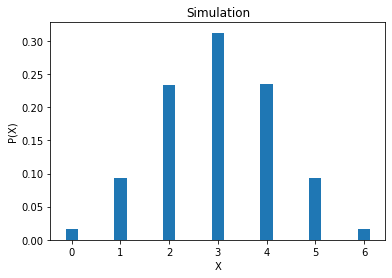
\includegraphics[width=0.58\textwidth]{assignment1.png}
\end{center}
\end{figure}
\end{Large}



\end{paracol}
\end{document}